% !TEX encoding = UTF-8
% !TEX TS-program = pdflatex
% !TEX root = ../tesi.tex

\subsection{UC1 - Autenticazione}
\begin{itemize}
  \item \textbf{Identificativo}: UC1
  \item \textbf{Nome}: autenticazione
  \item \textbf{Descrizione grafica}:
\end{itemize}

\begin{figure}[h]
  \centering
  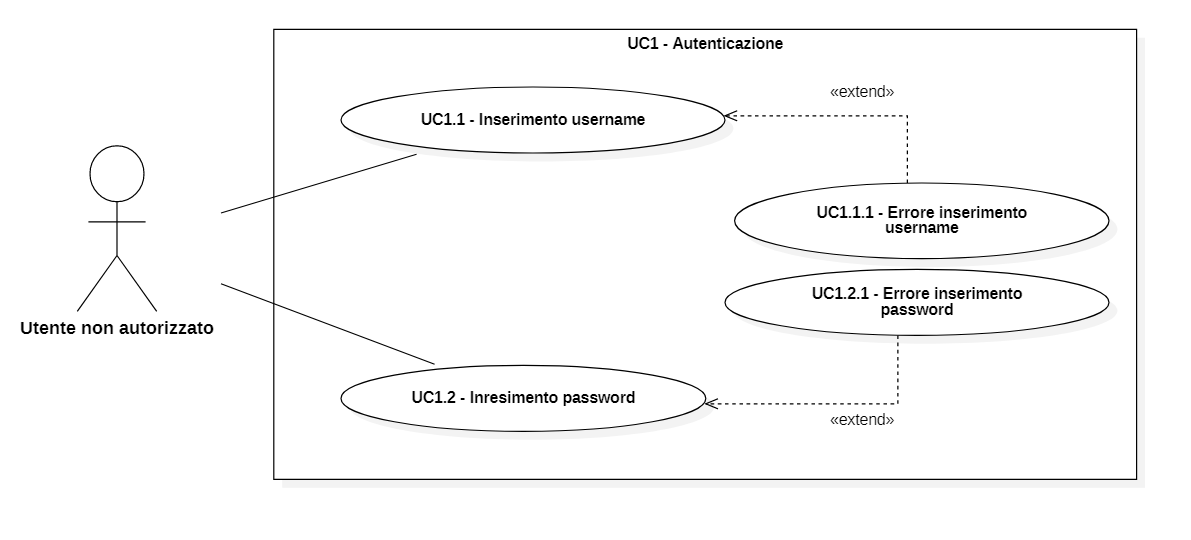
\includegraphics[scale=1.6]{immagini/usecase/UC1.png}
  \caption{Descrizione grafica caso d'uso UC1}
\end{figure}

\begin{itemize}
  \item \textbf{Attori}
        \begin{itemize}
          \item \textit{Primari}: utente non autorizzato
          \item \textit{Secondari}: Google o Faceebook (???)
        \end{itemize}
  \item \textbf{Precondizione}: l'utente non autenticato si trova sulla pagina di autenticazione.
  \item \textbf{Postcondizione}: l'utente è autenticato.
  \item \textbf{Scenario principale}: l'utente vuole effettuare il login all'applicazione.
  \item \textbf{Scenario secondario}: l'utente non riesce ad autenticarsi a causa di un errore nella procedura. (\textbf{UC1.3})
\end{itemize}

\subsubsection{UC1.1 - Inserimento username}
\begin{itemize}
  \item \textbf{Identificativo}: UC1.1
  \item \textbf{Nome}: inserimento username
  \item \textbf{Descrizione grafica}: (approfondita in UC1)
  \item \textbf{Attori}
        \begin{itemize}
          \item \textit{Primari}: utente non autorizzato
        \end{itemize}
  \item \textbf{Precondizione}: l'utente ha a disposizione una username
  \item \textbf{Postcondizione}: l'utente ha inserito la username.
  \item \textbf{Scenario principale}: l'utente inserisce la username nell'apposito campo di input.
  \item \textbf{Scenario secondario}: l'utente ha inserito una username non corretta che causa un errore. (\textbf{UC1.3})
\end{itemize}

\subsubsection{UC1.1.1 - Errore inserimento username}
\begin{itemize}
  \item \textbf{Identificativo}: UC1.1.1
  \item \textbf{Nome}: errore inserimento username
  \item \textbf{Descrizione grafica}: (approfondita in UC1)
  \item \textbf{Attori}
        \begin{itemize}
          \item \textit{Primari}: utente non autorizzato
        \end{itemize}
  \item \textbf{Precondizione}: la username inserita dall'utente non è correttta.
  \item \textbf{Postcondizione}: l'errore viene mostrato all'utente.
  \item \textbf{Scenario principale}: l'utente inserisce una username non corretta, il sistema segnala l'errore all'utente e mostra nuovamente la maschera di login.
\end{itemize}

\subsubsection{UC1.2 - Inserimento password}
\begin{itemize}
  \item \textbf{Identificativo}: UC1.1
  \item \textbf{Nome}: inserimento password
  \item \textbf{Descrizione grafica}: (approfondita in UC1)
  \item \textbf{Attori}
        \begin{itemize}
          \item \textit{Primari}: utente non autorizzato
        \end{itemize}
  \item \textbf{Precondizione}: l'utente ha a disposizione una password
  \item \textbf{Postcondizione}: l'utente ha inserito la password.
  \item \textbf{Scenario principale}: l'utente inserisce la password nell'apposito campo di input.
  \item \textbf{Scenario secondario}: l'utente ha inserito una password non corretta che causa un errore. (\textbf{UC1.3})
\end{itemize}

\subsubsection{UC1.2.1 - Errore inserimento password}
\begin{itemize}
  \item \textbf{Identificativo}: UC1.2.1
  \item \textbf{Nome}: errore inserimento password
  \item \textbf{Descrizione grafica}: (approfondita in UC1)
  \item \textbf{Attori}
        \begin{itemize}
          \item \textit{Primari}: utente non autorizzato
        \end{itemize}
  \item \textbf{Precondizione}: la password inserita dall'utente non è correttta.
  \item \textbf{Postcondizione}: l'errore viene mostrato all'utente.
  \item \textbf{Scenario principale}: l'utente inserisce una password non corretta, il sistema segnala l'errore all'utente e mostra nuovamente la maschera di login.
\end{itemize}

% \subsubsection{UC1.3 - Errore autenticazione}
% \begin{itemize}
%   \item \textbf{Identificativo}: UC1.3
%   \item \textbf{Nome}: errore autenticazione
%   \item \textbf{Descrizione grafica}: (approfondita in UC1)
%   \item \textbf{Attori}
%         \begin{itemize}
%           \item \textit{Primari}: utente non autorizzato
%         \end{itemize}
%   \item \textbf{Precondizione}: il sitema di autenticazione riceve la richiesta da parte dell'utente.
%   \item \textbf{Postcondizione}: il sistema comunica all'utente l'errore avvenuto, viene riproposta la maschera di login.
%   \item \textbf{Scenario principale}: la richiesta di autenticazione non viene gestita dal sistema che comunica l'errore avvenuto all'utente e mostra nuovamente la maschera di login per un nuovo tentativo.
% \end{itemize}
\newpage